% Options for packages loaded elsewhere
\PassOptionsToPackage{unicode}{hyperref}
\PassOptionsToPackage{hyphens}{url}
\PassOptionsToPackage{dvipsnames,svgnames,x11names}{xcolor}
%
\documentclass[
  letterpaper,
  DIV=11,
  numbers=noendperiod]{scrartcl}

\usepackage{amsmath,amssymb}
\usepackage{iftex}
\ifPDFTeX
  \usepackage[T1]{fontenc}
  \usepackage[utf8]{inputenc}
  \usepackage{textcomp} % provide euro and other symbols
\else % if luatex or xetex
  \usepackage{unicode-math}
  \defaultfontfeatures{Scale=MatchLowercase}
  \defaultfontfeatures[\rmfamily]{Ligatures=TeX,Scale=1}
\fi
\usepackage{lmodern}
\ifPDFTeX\else  
    % xetex/luatex font selection
\fi
% Use upquote if available, for straight quotes in verbatim environments
\IfFileExists{upquote.sty}{\usepackage{upquote}}{}
\IfFileExists{microtype.sty}{% use microtype if available
  \usepackage[]{microtype}
  \UseMicrotypeSet[protrusion]{basicmath} % disable protrusion for tt fonts
}{}
\makeatletter
\@ifundefined{KOMAClassName}{% if non-KOMA class
  \IfFileExists{parskip.sty}{%
    \usepackage{parskip}
  }{% else
    \setlength{\parindent}{0pt}
    \setlength{\parskip}{6pt plus 2pt minus 1pt}}
}{% if KOMA class
  \KOMAoptions{parskip=half}}
\makeatother
\usepackage{xcolor}
\setlength{\emergencystretch}{3em} % prevent overfull lines
\setcounter{secnumdepth}{5}
% Make \paragraph and \subparagraph free-standing
\makeatletter
\ifx\paragraph\undefined\else
  \let\oldparagraph\paragraph
  \renewcommand{\paragraph}{
    \@ifstar
      \xxxParagraphStar
      \xxxParagraphNoStar
  }
  \newcommand{\xxxParagraphStar}[1]{\oldparagraph*{#1}\mbox{}}
  \newcommand{\xxxParagraphNoStar}[1]{\oldparagraph{#1}\mbox{}}
\fi
\ifx\subparagraph\undefined\else
  \let\oldsubparagraph\subparagraph
  \renewcommand{\subparagraph}{
    \@ifstar
      \xxxSubParagraphStar
      \xxxSubParagraphNoStar
  }
  \newcommand{\xxxSubParagraphStar}[1]{\oldsubparagraph*{#1}\mbox{}}
  \newcommand{\xxxSubParagraphNoStar}[1]{\oldsubparagraph{#1}\mbox{}}
\fi
\makeatother

\usepackage{color}
\usepackage{fancyvrb}
\newcommand{\VerbBar}{|}
\newcommand{\VERB}{\Verb[commandchars=\\\{\}]}
\DefineVerbatimEnvironment{Highlighting}{Verbatim}{commandchars=\\\{\}}
% Add ',fontsize=\small' for more characters per line
\usepackage{framed}
\definecolor{shadecolor}{RGB}{241,243,245}
\newenvironment{Shaded}{\begin{snugshade}}{\end{snugshade}}
\newcommand{\AlertTok}[1]{\textcolor[rgb]{0.68,0.00,0.00}{#1}}
\newcommand{\AnnotationTok}[1]{\textcolor[rgb]{0.37,0.37,0.37}{#1}}
\newcommand{\AttributeTok}[1]{\textcolor[rgb]{0.40,0.45,0.13}{#1}}
\newcommand{\BaseNTok}[1]{\textcolor[rgb]{0.68,0.00,0.00}{#1}}
\newcommand{\BuiltInTok}[1]{\textcolor[rgb]{0.00,0.23,0.31}{#1}}
\newcommand{\CharTok}[1]{\textcolor[rgb]{0.13,0.47,0.30}{#1}}
\newcommand{\CommentTok}[1]{\textcolor[rgb]{0.37,0.37,0.37}{#1}}
\newcommand{\CommentVarTok}[1]{\textcolor[rgb]{0.37,0.37,0.37}{\textit{#1}}}
\newcommand{\ConstantTok}[1]{\textcolor[rgb]{0.56,0.35,0.01}{#1}}
\newcommand{\ControlFlowTok}[1]{\textcolor[rgb]{0.00,0.23,0.31}{\textbf{#1}}}
\newcommand{\DataTypeTok}[1]{\textcolor[rgb]{0.68,0.00,0.00}{#1}}
\newcommand{\DecValTok}[1]{\textcolor[rgb]{0.68,0.00,0.00}{#1}}
\newcommand{\DocumentationTok}[1]{\textcolor[rgb]{0.37,0.37,0.37}{\textit{#1}}}
\newcommand{\ErrorTok}[1]{\textcolor[rgb]{0.68,0.00,0.00}{#1}}
\newcommand{\ExtensionTok}[1]{\textcolor[rgb]{0.00,0.23,0.31}{#1}}
\newcommand{\FloatTok}[1]{\textcolor[rgb]{0.68,0.00,0.00}{#1}}
\newcommand{\FunctionTok}[1]{\textcolor[rgb]{0.28,0.35,0.67}{#1}}
\newcommand{\ImportTok}[1]{\textcolor[rgb]{0.00,0.46,0.62}{#1}}
\newcommand{\InformationTok}[1]{\textcolor[rgb]{0.37,0.37,0.37}{#1}}
\newcommand{\KeywordTok}[1]{\textcolor[rgb]{0.00,0.23,0.31}{\textbf{#1}}}
\newcommand{\NormalTok}[1]{\textcolor[rgb]{0.00,0.23,0.31}{#1}}
\newcommand{\OperatorTok}[1]{\textcolor[rgb]{0.37,0.37,0.37}{#1}}
\newcommand{\OtherTok}[1]{\textcolor[rgb]{0.00,0.23,0.31}{#1}}
\newcommand{\PreprocessorTok}[1]{\textcolor[rgb]{0.68,0.00,0.00}{#1}}
\newcommand{\RegionMarkerTok}[1]{\textcolor[rgb]{0.00,0.23,0.31}{#1}}
\newcommand{\SpecialCharTok}[1]{\textcolor[rgb]{0.37,0.37,0.37}{#1}}
\newcommand{\SpecialStringTok}[1]{\textcolor[rgb]{0.13,0.47,0.30}{#1}}
\newcommand{\StringTok}[1]{\textcolor[rgb]{0.13,0.47,0.30}{#1}}
\newcommand{\VariableTok}[1]{\textcolor[rgb]{0.07,0.07,0.07}{#1}}
\newcommand{\VerbatimStringTok}[1]{\textcolor[rgb]{0.13,0.47,0.30}{#1}}
\newcommand{\WarningTok}[1]{\textcolor[rgb]{0.37,0.37,0.37}{\textit{#1}}}

\providecommand{\tightlist}{%
  \setlength{\itemsep}{0pt}\setlength{\parskip}{0pt}}\usepackage{longtable,booktabs,array}
\usepackage{calc} % for calculating minipage widths
% Correct order of tables after \paragraph or \subparagraph
\usepackage{etoolbox}
\makeatletter
\patchcmd\longtable{\par}{\if@noskipsec\mbox{}\fi\par}{}{}
\makeatother
% Allow footnotes in longtable head/foot
\IfFileExists{footnotehyper.sty}{\usepackage{footnotehyper}}{\usepackage{footnote}}
\makesavenoteenv{longtable}
\usepackage{graphicx}
\makeatletter
\def\maxwidth{\ifdim\Gin@nat@width>\linewidth\linewidth\else\Gin@nat@width\fi}
\def\maxheight{\ifdim\Gin@nat@height>\textheight\textheight\else\Gin@nat@height\fi}
\makeatother
% Scale images if necessary, so that they will not overflow the page
% margins by default, and it is still possible to overwrite the defaults
% using explicit options in \includegraphics[width, height, ...]{}
\setkeys{Gin}{width=\maxwidth,height=\maxheight,keepaspectratio}
% Set default figure placement to htbp
\makeatletter
\def\fps@figure{htbp}
\makeatother

\KOMAoption{captions}{tableheading}
\makeatletter
\@ifpackageloaded{tcolorbox}{}{\usepackage[skins,breakable]{tcolorbox}}
\@ifpackageloaded{fontawesome5}{}{\usepackage{fontawesome5}}
\definecolor{quarto-callout-color}{HTML}{909090}
\definecolor{quarto-callout-note-color}{HTML}{0758E5}
\definecolor{quarto-callout-important-color}{HTML}{CC1914}
\definecolor{quarto-callout-warning-color}{HTML}{EB9113}
\definecolor{quarto-callout-tip-color}{HTML}{00A047}
\definecolor{quarto-callout-caution-color}{HTML}{FC5300}
\definecolor{quarto-callout-color-frame}{HTML}{acacac}
\definecolor{quarto-callout-note-color-frame}{HTML}{4582ec}
\definecolor{quarto-callout-important-color-frame}{HTML}{d9534f}
\definecolor{quarto-callout-warning-color-frame}{HTML}{f0ad4e}
\definecolor{quarto-callout-tip-color-frame}{HTML}{02b875}
\definecolor{quarto-callout-caution-color-frame}{HTML}{fd7e14}
\makeatother
\makeatletter
\@ifpackageloaded{caption}{}{\usepackage{caption}}
\AtBeginDocument{%
\ifdefined\contentsname
  \renewcommand*\contentsname{Table of contents}
\else
  \newcommand\contentsname{Table of contents}
\fi
\ifdefined\listfigurename
  \renewcommand*\listfigurename{List of Figures}
\else
  \newcommand\listfigurename{List of Figures}
\fi
\ifdefined\listtablename
  \renewcommand*\listtablename{List of Tables}
\else
  \newcommand\listtablename{List of Tables}
\fi
\ifdefined\figurename
  \renewcommand*\figurename{Figure}
\else
  \newcommand\figurename{Figure}
\fi
\ifdefined\tablename
  \renewcommand*\tablename{Table}
\else
  \newcommand\tablename{Table}
\fi
}
\@ifpackageloaded{float}{}{\usepackage{float}}
\floatstyle{ruled}
\@ifundefined{c@chapter}{\newfloat{codelisting}{h}{lop}}{\newfloat{codelisting}{h}{lop}[chapter]}
\floatname{codelisting}{Listing}
\newcommand*\listoflistings{\listof{codelisting}{List of Listings}}
\makeatother
\makeatletter
\makeatother
\makeatletter
\@ifpackageloaded{caption}{}{\usepackage{caption}}
\@ifpackageloaded{subcaption}{}{\usepackage{subcaption}}
\makeatother

\ifLuaTeX
  \usepackage{selnolig}  % disable illegal ligatures
\fi
\usepackage{bookmark}

\IfFileExists{xurl.sty}{\usepackage{xurl}}{} % add URL line breaks if available
\urlstyle{same} % disable monospaced font for URLs
\hypersetup{
  pdftitle={A sample workflow},
  pdfauthor={Victor; Jonathan; Lizzie},
  colorlinks=true,
  linkcolor={blue},
  filecolor={Maroon},
  citecolor={Blue},
  urlcolor={Blue},
  pdfcreator={LaTeX via pandoc}}


\title{A sample workflow}
\author{Victor \and Jonathan \and Lizzie}
\date{April 2025}

\begin{document}
\maketitle

\renewcommand*\contentsname{Table of contents}
{
\hypersetup{linkcolor=}
\setcounter{tocdepth}{3}
\tableofcontents
}

To show our workflow in action, we examine a subset of the Living Planet
Index (LPI, download at: https://www.livingplanetindex.org/data\_portal.
This download should include a csv file, here: LPD\_2024\_public.csv,
that we use below). We discuss the LPI in the main text; for more
information, check out \href{www.livingplanetindex.org/}{their website}.

\section{Step 1: Research question}\label{step-1-research-question}

Here we need to focus on exactly what question we are trying to answer,
which will guide us in the next steps. This step is sometimes skipped
over or moved through so quickly that the exact question is not clear,
but is critical for developing a useful model. Many early papers on the
LPI seem focused on something similar to: Are vertebrate species overall
declining on average? And, if so, by how much? We, however, might want
to have a question that more clearly allows any directionality, so we
could start with: What is the global trend for biodiversity in vetebrate
species? This is rather broad and might mean we should develop a model
that will yield one global estimate. In thinking about this, we would
likely realize we don't want just that, we actually want to understand
the variation across different species and perhaps populations and also
have a global estimate. So we might refine the question to:

\begin{tcolorbox}[enhanced jigsaw, left=2mm, toprule=.15mm, leftrule=.75mm, rightrule=.15mm, breakable, colframe=quarto-callout-tip-color-frame, colback=white, opacityback=0, arc=.35mm, bottomrule=.15mm]

What is the global trend over time in vertebrate species population
numbers, both overall and how does it vary across species and
populations?

\end{tcolorbox}

\begin{Shaded}
\begin{Highlighting}[]
\NormalTok{wd }\OtherTok{\textless{}{-}} \StringTok{"/home/victor/projects/forecastflows/analyses"}

\FunctionTok{set.seed}\NormalTok{(}\DecValTok{20012029}\NormalTok{)}

\FunctionTok{suppressPackageStartupMessages}\NormalTok{(}\FunctionTok{library}\NormalTok{(rstan))}
\FunctionTok{library}\NormalTok{(ggplot2)}

\NormalTok{lpi\_data }\OtherTok{\textless{}{-}} \FunctionTok{read.csv}\NormalTok{(}\FunctionTok{file.path}\NormalTok{(wd, }\StringTok{"input"}\NormalTok{, }\StringTok{"LPD\_2024\_public.csv"}\NormalTok{), }\AttributeTok{header=}\NormalTok{T)}
\end{Highlighting}
\end{Shaded}

\section{Step 2: Model building}\label{step-2-model-building}

Next we need to think about how we would build a model to address this
question, with the goal to build the model and evaluate it using
simulated data. There are a lot of demographic models in population
ecology, so we might revisit those and consider a discrete time model
based on population size and stepping through each year of data. We
might also start with a simple linear model, where populations can go
up, down or do nothing.

Using a simple linear gets us started, but now we need to consider how
we will model species and populations. Populations usually are nested in
species in ecological models, so we might consider that to start. In
this first hierarchical model, we thus assume that populations are
exchangeable---an assumption we might refine later. We also need to make
sure our model yields one global estimate; for this we decide to model
species trends over time as part of larger distribution. Our resulting
model would then be:

\[\log(y_i) \sim \text{normal}(\mu_i, \ \sigma)\]

\[\mu_i = \alpha_{\text{pop}[\text{sp}[i]]} + \beta_{\text{pop}[\text{sp}[i]]} * \text{year}_i\]

\[\alpha_{\text{pop}[\text{sp}]}  \sim \text{normal}(\mu_{\alpha, \text{sp}}, \ \sigma_{\alpha, \text{sp}})
\quad \mu_{\alpha,\text{sp}} \sim \text{normal}(\mu_{\alpha_1}, \ \sigma_{\alpha_1}) 
\quad \sigma_{\alpha,\text{sp}} \sim \text{normal}(\mu_{\alpha_2}, \ \sigma_{\alpha_2}) \]

\[\beta_{\text{pop}[\text{sp}]}  \sim \text{normal}(\mu_{\beta, \text{sp}}, \ \sigma_{\beta, \text{sp}}) 
\quad \mu_{\beta,\text{sp}} \sim \text{normal}(\mu_{\beta_1}, \ \sigma_{\beta_1}) 
\quad \sigma_{\beta,\text{sp}} \sim \text{normal}(\mu_{\beta_2}, \ \sigma_{\beta_2}) \]

(where all the \(\sigma\) parameters are greater than zero)

\section{Step 3: Model evaluation}\label{step-3-model-evaluation}

Now we need to simulate data to test our model. As we start to think
about how to do this, we may become overwhelmed with the scale of the
question we started with. We likely would not feel immediately sure how
to simulate for all different vertebrate species. For example, what are
reasonable starting population sizes (intercepts) for different groups?
As we start to answer this we likely would realize different clades
should have different starting population sizes. We could thus try to
build in increasing complexity immediately, but then we will likely
struggle to see how our model is performing at the scales we care about
-- for each population in each species. It is almost always better to
scale back the question (and potentially dataset) when confronted with
these sorts of problems.

\subsection{Stepping backward\ldots{}}\label{stepping-backward}

Here we would likely feedback (step back) one to two steps. We could
step back to Step 2 and consider adding a phylogeny or other structure
from which we could then simulate data from, or we could step back to
Step 1 and narrow the question (before potentially building it back up.)
As mentioned above, we believe the latter approach is usually better as
working on a small scale first can point out more fundamental problems
versus starting big and then spending much longer to identify
fundamental problems (or potentially missing them).

So here we refine our question to:

\begin{tcolorbox}[enhanced jigsaw, left=2mm, toprule=.15mm, leftrule=.75mm, rightrule=.15mm, breakable, colframe=quarto-callout-tip-color-frame, colback=white, opacityback=0, arc=.35mm, bottomrule=.15mm]

What is trend in mammal species population numbers in southern Africa,
both overall and how does it vary across species and populations?

\end{tcolorbox}

We chose this because mammals are a well studied group compared to other
clades/groups in the dataset, so we will have a better idea of how to
simulate data, and whether our model makes sense.

\begin{Shaded}
\begin{Highlighting}[]
\NormalTok{lpi\_subset }\OtherTok{\textless{}{-}}\FunctionTok{subset}\NormalTok{(lpi\_data, Region }\SpecialCharTok{==} \StringTok{"Africa"} \SpecialCharTok{\&}\NormalTok{ Class }\SpecialCharTok{==} \StringTok{"Mammalia"} \SpecialCharTok{\&} 
\NormalTok{                      Included.in.LPR2024 }\SpecialCharTok{==} \DecValTok{1}\NormalTok{ )}

\CommentTok{\# subset 5+ counts}
\NormalTok{obs.cnt}\OtherTok{\textless{}{-}}\ConstantTok{NULL}
\ControlFlowTok{for}\NormalTok{ (n }\ControlFlowTok{in} \DecValTok{1}\SpecialCharTok{:}\FunctionTok{dim}\NormalTok{(lpi\_subset)[}\DecValTok{1}\NormalTok{])\{}
\NormalTok{  obs.cnt[n]}\OtherTok{\textless{}{-}}\FunctionTok{sum}\NormalTok{(lpi\_subset[n, }\DecValTok{31}\SpecialCharTok{:}\DecValTok{101}\NormalTok{]}\SpecialCharTok{!=}\StringTok{"NULL"}\NormalTok{)}
\NormalTok{\}}
\NormalTok{lpi\_subset}\OtherTok{\textless{}{-}}\NormalTok{lpi\_subset[obs.cnt}\SpecialCharTok{\textgreater{}}\DecValTok{4}\NormalTok{,]}

\CommentTok{\# subset species 10+ populations}
\NormalTok{sp }\OtherTok{\textless{}{-}} \FunctionTok{unique}\NormalTok{(lpi\_subset}\SpecialCharTok{$}\NormalTok{Binomial)}
\NormalTok{sp.cnt}\OtherTok{\textless{}{-}}\ConstantTok{NULL}
\ControlFlowTok{for}\NormalTok{(x }\ControlFlowTok{in} \DecValTok{1}\SpecialCharTok{:}\FunctionTok{length}\NormalTok{(sp))\{}
\NormalTok{  Af.tmp}\OtherTok{\textless{}{-}}\FunctionTok{subset}\NormalTok{(lpi\_subset, Binomial }\SpecialCharTok{==}\NormalTok{ sp[x])}
\NormalTok{  sp.cnt[x]}\OtherTok{\textless{}{-}}\FunctionTok{dim}\NormalTok{(Af.tmp)[}\DecValTok{1}\NormalTok{]}
\NormalTok{\}}
\NormalTok{keep.sp}\OtherTok{\textless{}{-}}\NormalTok{sp[sp.cnt}\SpecialCharTok{\textgreater{}}\DecValTok{9}\NormalTok{]}
\NormalTok{lpi\_subset}\OtherTok{\textless{}{-}}\NormalTok{lpi\_subset[lpi\_subset}\SpecialCharTok{$}\NormalTok{Binomial }\SpecialCharTok{\%in\%}\NormalTok{ keep.sp,]}
\end{Highlighting}
\end{Shaded}

\subsection{Simulating data}\label{simulating-data}

Now we start to simulate! We follow the mathematical model we built
above and simulate data from it.

\begin{Shaded}
\begin{Highlighting}[]
\NormalTok{nspecies }\OtherTok{\textless{}{-}} \DecValTok{9} \CommentTok{\# no. of species}
\NormalTok{npops\_persp }\OtherTok{\textless{}{-}} \FunctionTok{round}\NormalTok{(}\FunctionTok{runif}\NormalTok{(nspecies, }\DecValTok{2}\NormalTok{, }\DecValTok{15}\NormalTok{)) }\CommentTok{\# no. of different populations per species}
\NormalTok{npops }\OtherTok{\textless{}{-}} \FunctionTok{sum}\NormalTok{(npops\_persp) }\CommentTok{\# total no. of different populations}
\NormalTok{nobs\_perpop }\OtherTok{\textless{}{-}} \FunctionTok{round}\NormalTok{(}\FunctionTok{runif}\NormalTok{(npops, }\DecValTok{20}\NormalTok{, }\DecValTok{60}\NormalTok{)) }\CommentTok{\# no. of different observations per population}

\NormalTok{spid\_perpop }\OtherTok{\textless{}{-}} \FunctionTok{rep}\NormalTok{(}\DecValTok{1}\SpecialCharTok{:}\NormalTok{nspecies, }\AttributeTok{times =}\NormalTok{ npops\_persp)}
\NormalTok{spid\_perobs }\OtherTok{\textless{}{-}} \FunctionTok{rep}\NormalTok{(spid\_perpop, }\AttributeTok{times =}\NormalTok{ nobs\_perpop)}
\NormalTok{popid\_perobs }\OtherTok{\textless{}{-}} \FunctionTok{rep}\NormalTok{(}\DecValTok{1}\SpecialCharTok{:}\NormalTok{npops, }\AttributeTok{times =}\NormalTok{ nobs\_perpop)}

\NormalTok{years }\OtherTok{\textless{}{-}} \FunctionTok{c}\NormalTok{()}
\ControlFlowTok{for}\NormalTok{(np }\ControlFlowTok{in}\NormalTok{ nobs\_perpop)\{}
\NormalTok{  years\_p }\OtherTok{\textless{}{-}} \FunctionTok{sample}\NormalTok{(}\DecValTok{1950}\SpecialCharTok{:}\DecValTok{2020}\NormalTok{, }\AttributeTok{size =}\NormalTok{ np, }\AttributeTok{replace =} \ConstantTok{FALSE}\NormalTok{)}
\NormalTok{  years }\OtherTok{\textless{}{-}} \FunctionTok{c}\NormalTok{(years, years\_p)}
\NormalTok{\}}

\CommentTok{\# nested intercepts}
\NormalTok{mu\_alpha1 }\OtherTok{\textless{}{-}} \FunctionTok{log}\NormalTok{(}\DecValTok{200}\NormalTok{)}
\NormalTok{sigma\_alpha1 }\OtherTok{\textless{}{-}}  \FunctionTok{log}\NormalTok{(}\DecValTok{50}\NormalTok{)}\SpecialCharTok{/}\FloatTok{2.57}
\NormalTok{mu\_alpha\_sp }\OtherTok{\textless{}{-}} \FunctionTok{rnorm}\NormalTok{(}\AttributeTok{n =}\NormalTok{ nspecies, }\AttributeTok{mean =}\NormalTok{ mu\_alpha1, }\AttributeTok{sd =}\NormalTok{ sigma\_alpha1)}
\NormalTok{mu\_alpha2 }\OtherTok{\textless{}{-}} \FunctionTok{log}\NormalTok{(}\DecValTok{20}\NormalTok{)}
\NormalTok{sigma\_alpha2 }\OtherTok{\textless{}{-}} \FunctionTok{log}\NormalTok{(}\DecValTok{50}\NormalTok{)}\SpecialCharTok{/}\FloatTok{2.57}
\NormalTok{sig\_species\_alpha }\OtherTok{\textless{}{-}} \FunctionTok{abs}\NormalTok{(}\FunctionTok{rnorm}\NormalTok{(}\AttributeTok{n =}\NormalTok{ nspecies, }\AttributeTok{mean =}\NormalTok{ mu\_alpha2, }
                               \AttributeTok{sd =}\NormalTok{ sigma\_alpha2))}
\NormalTok{alpha\_pop\_sp }\OtherTok{\textless{}{-}} \FunctionTok{rnorm}\NormalTok{(}\AttributeTok{n =}\NormalTok{ npops, }\AttributeTok{mean =}\NormalTok{ mu\_alpha\_sp[spid\_perpop], }
                      \AttributeTok{sd =}\NormalTok{ sig\_species\_alpha[spid\_perpop]) }

\CommentTok{\# nested slopes}
\NormalTok{mu\_beta1 }\OtherTok{\textless{}{-}} \FloatTok{0.05}
\NormalTok{sigma\_beta1 }\OtherTok{\textless{}{-}} \FloatTok{0.25}\SpecialCharTok{/}\FloatTok{2.57}
\NormalTok{mu\_beta\_sp }\OtherTok{\textless{}{-}} \FunctionTok{rnorm}\NormalTok{(}\AttributeTok{n =}\NormalTok{ nspecies, }\AttributeTok{mean =}\NormalTok{ mu\_beta1, }\AttributeTok{sd =}\NormalTok{ sigma\_beta1)}
\NormalTok{mu\_beta2 }\OtherTok{\textless{}{-}} \DecValTok{0}
\NormalTok{sigma\_beta2 }\OtherTok{\textless{}{-}} \FloatTok{0.05}\SpecialCharTok{/}\FloatTok{2.57}
\NormalTok{sig\_species\_beta }\OtherTok{\textless{}{-}} \FunctionTok{abs}\NormalTok{(}\FunctionTok{rnorm}\NormalTok{(}\AttributeTok{n =}\NormalTok{ nspecies, }\AttributeTok{mean =}\NormalTok{ mu\_beta2, }
                              \AttributeTok{sd =}\NormalTok{ sigma\_beta2))}
\NormalTok{beta\_pop\_sp }\OtherTok{\textless{}{-}} \FunctionTok{rnorm}\NormalTok{(}\AttributeTok{n =}\NormalTok{ npops, }\AttributeTok{mean =}\NormalTok{ mu\_beta\_sp[spid\_perpop], }
                     \AttributeTok{sd =}\NormalTok{ sig\_species\_beta[spid\_perpop]) }

\CommentTok{\# save simulated intercepts and slopes}
\NormalTok{pops\_fit }\OtherTok{\textless{}{-}} \FunctionTok{data.frame}\NormalTok{()}
\NormalTok{pid }\OtherTok{\textless{}{-}} \DecValTok{1}
\ControlFlowTok{for}\NormalTok{(sp }\ControlFlowTok{in} \DecValTok{1}\SpecialCharTok{:}\NormalTok{nspecies)\{}
  \ControlFlowTok{for}\NormalTok{(p }\ControlFlowTok{in} \DecValTok{1}\SpecialCharTok{:}\NormalTok{npops\_persp[sp])\{}
\NormalTok{    pops\_fit }\OtherTok{\textless{}{-}} \FunctionTok{rbind}\NormalTok{(pops\_fit, }\FunctionTok{data.frame}\NormalTok{(}\AttributeTok{species =}\NormalTok{ sp, }\AttributeTok{pop =}\NormalTok{ pid))}
\NormalTok{    pid }\OtherTok{\textless{}{-}}\NormalTok{ pid }\SpecialCharTok{+} \DecValTok{1}
\NormalTok{  \}}
\NormalTok{\}}
\NormalTok{pops\_fit}\SpecialCharTok{$}\NormalTok{int }\OtherTok{\textless{}{-}}\NormalTok{ alpha\_pop\_sp}
\NormalTok{pops\_fit}\SpecialCharTok{$}\NormalTok{slp }\OtherTok{\textless{}{-}}\NormalTok{ beta\_pop\_sp}

\NormalTok{sigma\_obs }\OtherTok{\textless{}{-}} \FloatTok{0.75} \CommentTok{\# common observational error}

\NormalTok{y }\OtherTok{\textless{}{-}} \FunctionTok{c}\NormalTok{()}
\ControlFlowTok{for}\NormalTok{(p }\ControlFlowTok{in} \DecValTok{1}\SpecialCharTok{:}\NormalTok{npops)\{}
\NormalTok{  nobs\_p }\OtherTok{\textless{}{-}}\NormalTok{ nobs\_perpop[p]}
\NormalTok{  alpha\_p }\OtherTok{\textless{}{-}}\NormalTok{ alpha\_pop\_sp[p]}
\NormalTok{  beta\_p }\OtherTok{\textless{}{-}}\NormalTok{ beta\_pop\_sp[p]}
  
\NormalTok{  years\_p }\OtherTok{\textless{}{-}}\NormalTok{ years[popid\_perobs }\SpecialCharTok{==}\NormalTok{ p] }
  
\NormalTok{  yhat\_p }\OtherTok{\textless{}{-}}\NormalTok{ alpha\_p }\SpecialCharTok{+}\NormalTok{ beta\_p }\SpecialCharTok{*}\NormalTok{ (years\_p }\SpecialCharTok{{-}} \DecValTok{1980}\NormalTok{)}
  \CommentTok{\# yhat\_p \textless{}{-} alpha\_p}
\NormalTok{  y\_p }\OtherTok{\textless{}{-}} \FunctionTok{exp}\NormalTok{(}\FunctionTok{rnorm}\NormalTok{(}\AttributeTok{n =}\NormalTok{ nobs\_p, }\AttributeTok{mean =}\NormalTok{ yhat\_p, }\AttributeTok{sd =}\NormalTok{ sigma\_obs))}
\NormalTok{  y }\OtherTok{\textless{}{-}} \FunctionTok{c}\NormalTok{(y, y\_p)}
\NormalTok{\}}


\NormalTok{datasim }\OtherTok{\textless{}{-}} \FunctionTok{data.frame}\NormalTok{(}
\NormalTok{  y, }
  \AttributeTok{year =}\NormalTok{ years }\SpecialCharTok{{-}} \DecValTok{1980}\NormalTok{,}
  \AttributeTok{species =} \FunctionTok{as.character}\NormalTok{(spid\_perobs),}
  \AttributeTok{population =} \FunctionTok{paste0}\NormalTok{(spid\_perobs,popid\_perobs)}
\NormalTok{)}

\NormalTok{datasim}\SpecialCharTok{$}\NormalTok{logy }\OtherTok{\textless{}{-}} \FunctionTok{log}\NormalTok{(datasim}\SpecialCharTok{$}\NormalTok{y)}

\FunctionTok{ggplot}\NormalTok{(}\AttributeTok{data =}\NormalTok{ datasim) }\SpecialCharTok{+}
  \FunctionTok{geom\_line}\NormalTok{(}\FunctionTok{aes}\NormalTok{(}\AttributeTok{x =}\NormalTok{ year}\SpecialCharTok{+}\DecValTok{1980}\NormalTok{, }\AttributeTok{y =}\NormalTok{ y, }
                \AttributeTok{group =}\NormalTok{ population,}
                \AttributeTok{color =}\NormalTok{ species)) }\SpecialCharTok{+}
  \FunctionTok{theme\_bw}\NormalTok{() }\SpecialCharTok{+}
  \FunctionTok{labs}\NormalTok{(}\AttributeTok{x =} \StringTok{\textquotesingle{}Year\textquotesingle{}}\NormalTok{, }\AttributeTok{y =} \StringTok{\textquotesingle{}Simulated counts\textquotesingle{}}\NormalTok{, }\AttributeTok{colour =} \StringTok{\textquotesingle{}Species\textquotesingle{}}\NormalTok{)}
\end{Highlighting}
\end{Shaded}

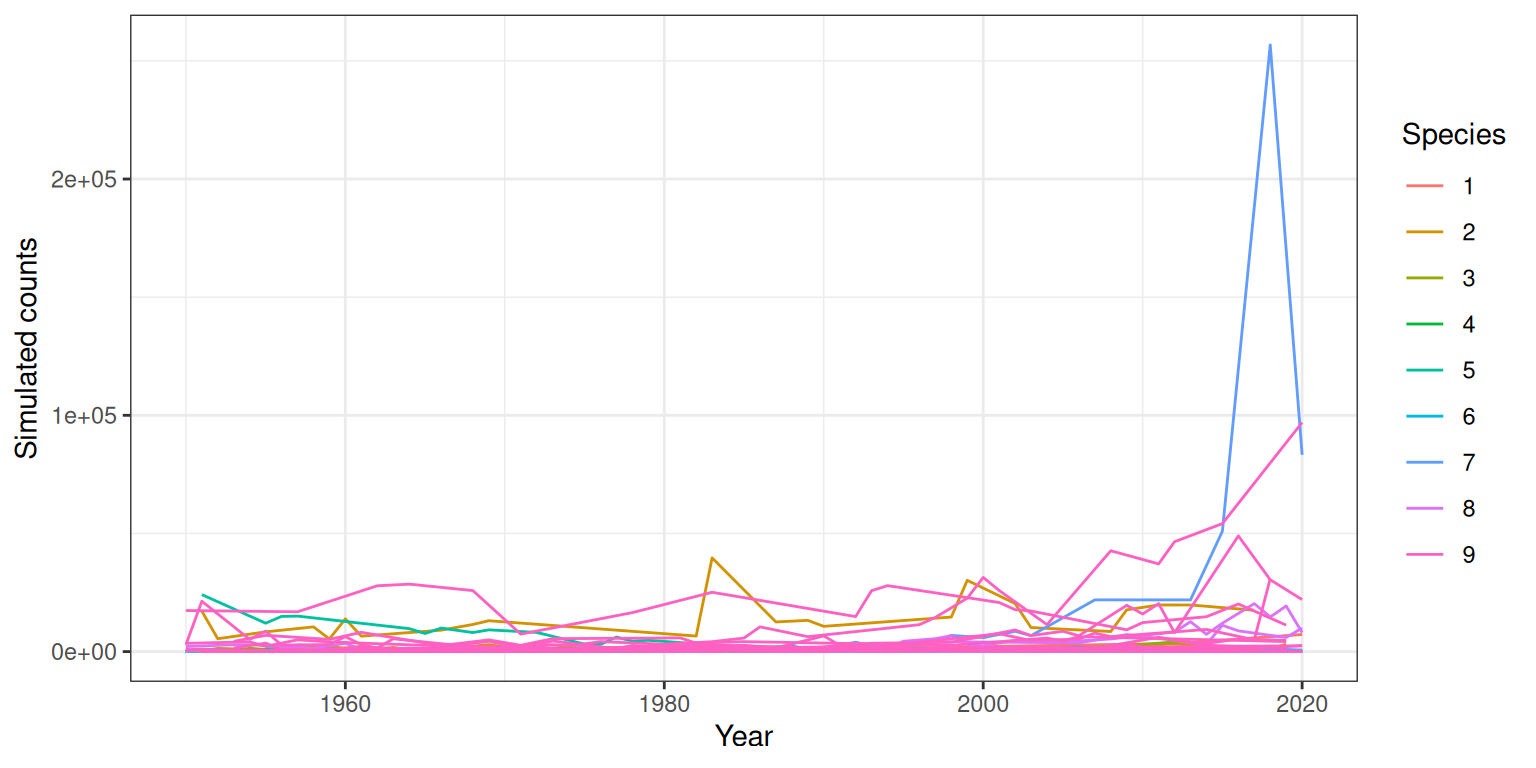
\includegraphics{lpiworkflow_files/figure-pdf/sim data-1.pdf}

\begin{Shaded}
\begin{Highlighting}[]
\FunctionTok{ggplot}\NormalTok{(}\AttributeTok{data =}\NormalTok{ datasim) }\SpecialCharTok{+}
  \FunctionTok{geom\_line}\NormalTok{(}\FunctionTok{aes}\NormalTok{(}\AttributeTok{x =}\NormalTok{ year}\SpecialCharTok{+}\DecValTok{1980}\NormalTok{, }\AttributeTok{y =}\NormalTok{ logy, }
                \AttributeTok{group =}\NormalTok{ population,}
                \AttributeTok{color =}\NormalTok{ species)) }\SpecialCharTok{+}
  \FunctionTok{theme\_bw}\NormalTok{() }\SpecialCharTok{+}
  \FunctionTok{labs}\NormalTok{(}\AttributeTok{x =} \StringTok{\textquotesingle{}Year\textquotesingle{}}\NormalTok{, }\AttributeTok{y =} \StringTok{\textquotesingle{}Simulated counts (log{-}scale)\textquotesingle{}}\NormalTok{, }\AttributeTok{colour =} \StringTok{\textquotesingle{}Species\textquotesingle{}}\NormalTok{)}
\end{Highlighting}
\end{Shaded}

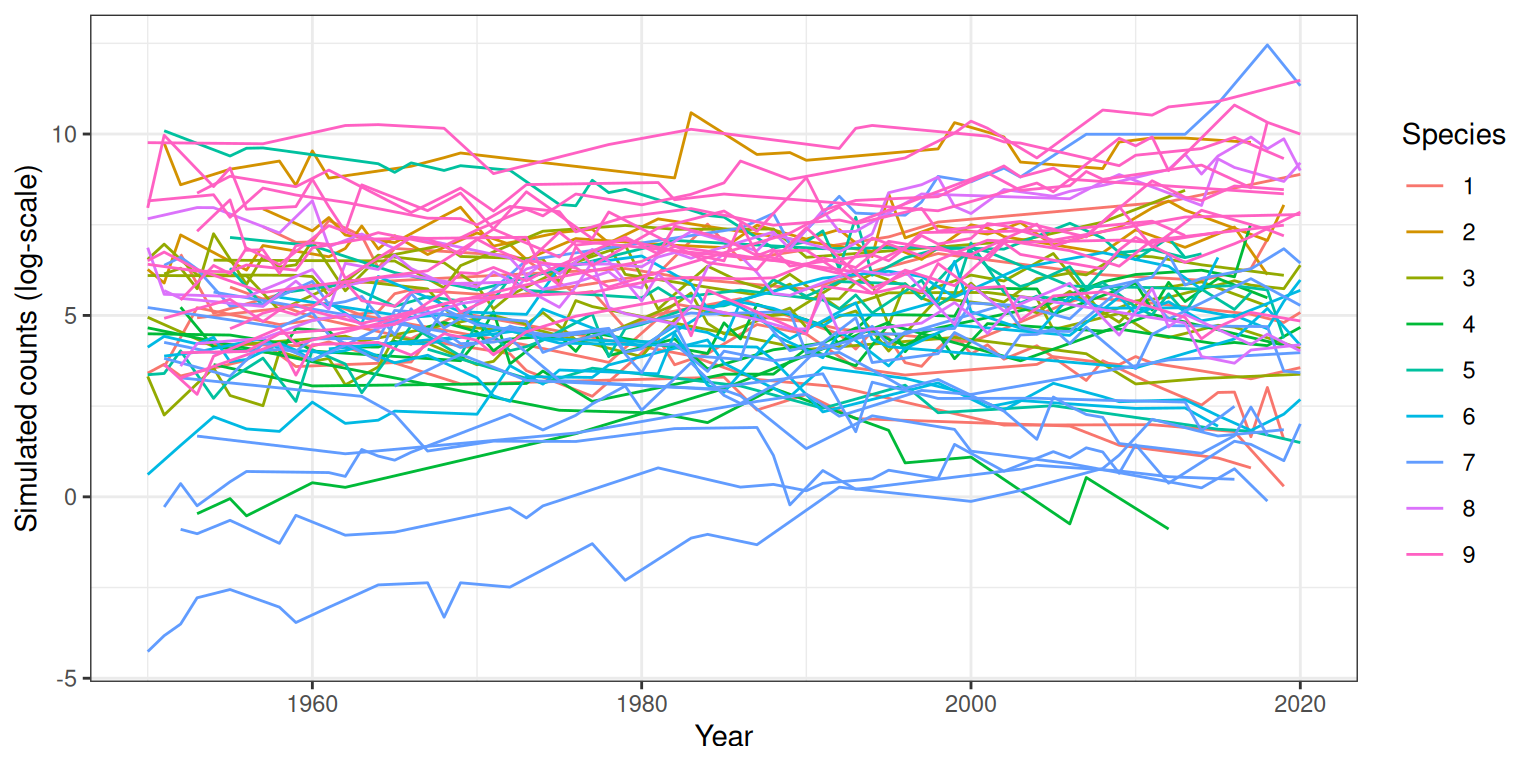
\includegraphics{lpiworkflow_files/figure-pdf/sim data-2.pdf}

\subsection{Fit and check model on simulated
data!}\label{fit-and-check-model-on-simulated-data}

Now we code the model from our mathematical notation (above) and fit it
to our simulated data (also built from our mathematical model).

\begin{Shaded}
\begin{Highlighting}[]

\KeywordTok{data}\NormalTok{ \{}
  \DataTypeTok{int}\NormalTok{\textless{}}\KeywordTok{lower}\NormalTok{=}\DecValTok{1}\NormalTok{\textgreater{} N;}
  \DataTypeTok{int}\NormalTok{\textless{}}\KeywordTok{lower}\NormalTok{=}\DecValTok{1}\NormalTok{\textgreater{} Nsp;}
  \DataTypeTok{int}\NormalTok{\textless{}}\KeywordTok{lower}\NormalTok{=}\DecValTok{1}\NormalTok{\textgreater{} Npop;}
  \DataTypeTok{vector}\NormalTok{[N] y;}
  \DataTypeTok{vector}\NormalTok{[N] year;}
  \DataTypeTok{array}\NormalTok{[Npop] }\DataTypeTok{int}\NormalTok{\textless{}}\KeywordTok{lower}\NormalTok{=}\DecValTok{1}\NormalTok{,}\KeywordTok{upper}\NormalTok{=Nsp\textgreater{} spid\_perpop;}
  \DataTypeTok{array}\NormalTok{[N] }\DataTypeTok{int}\NormalTok{\textless{}}\KeywordTok{lower}\NormalTok{=}\DecValTok{1}\NormalTok{,}\KeywordTok{upper}\NormalTok{=Npop\textgreater{} popid;}
\NormalTok{\}}

\KeywordTok{transformed data}\NormalTok{\{}
  \DataTypeTok{vector}\NormalTok{[N] logy = log(y);}
\NormalTok{\}}

\KeywordTok{parameters}\NormalTok{ \{}
  \DataTypeTok{real}\NormalTok{ mu\_alpha1; }\CommentTok{// overall species intercept}
  \DataTypeTok{real}\NormalTok{\textless{}}\KeywordTok{lower}\NormalTok{=}\DecValTok{0}\NormalTok{\textgreater{} sigma\_alpha1; }
  
  \DataTypeTok{real}\NormalTok{ mu\_alpha2;}
  \DataTypeTok{real}\NormalTok{\textless{}}\KeywordTok{lower}\NormalTok{=}\DecValTok{0}\NormalTok{\textgreater{} sigma\_alpha2;}
  
  \DataTypeTok{array}\NormalTok{[Nsp] }\DataTypeTok{real}\NormalTok{ mu\_alpha\_sp; }\CommentTok{// species{-}level intercepts}
  \DataTypeTok{array}\NormalTok{[Nsp] }\DataTypeTok{real}\NormalTok{\textless{}}\KeywordTok{lower}\NormalTok{=}\DecValTok{0}\NormalTok{\textgreater{} sig\_species\_alpha;}
  
  \DataTypeTok{array}\NormalTok{[Npop] }\DataTypeTok{real}\NormalTok{ alpha\_tilde\_pop\_sp; }\CommentTok{// non{-}centered population intercepts}
  
  \DataTypeTok{real}\NormalTok{ mu\_beta1; }\CommentTok{// overall species trend}
  \DataTypeTok{real}\NormalTok{\textless{}}\KeywordTok{lower}\NormalTok{=}\DecValTok{0}\NormalTok{\textgreater{} sigma\_beta1;}
  
  \DataTypeTok{real}\NormalTok{ mu\_beta2;}
  \DataTypeTok{real}\NormalTok{\textless{}}\KeywordTok{lower}\NormalTok{=}\DecValTok{0}\NormalTok{\textgreater{} sigma\_beta2;}
  
  \DataTypeTok{array}\NormalTok{[Nsp] }\DataTypeTok{real}\NormalTok{ mu\_beta\_sp; }\CommentTok{// species{-}level slopes}
  \DataTypeTok{array}\NormalTok{[Nsp] }\DataTypeTok{real}\NormalTok{\textless{}}\KeywordTok{lower}\NormalTok{=}\DecValTok{0}\NormalTok{\textgreater{} sig\_species\_beta;}
  
  \DataTypeTok{array}\NormalTok{[Npop] }\DataTypeTok{real}\NormalTok{ beta\_tilde\_pop\_sp; }\CommentTok{// non{-}centered population slopes}
  
  \DataTypeTok{real}\NormalTok{\textless{}}\KeywordTok{lower}\NormalTok{=}\DecValTok{0}\NormalTok{\textgreater{} sigma;}
   
\NormalTok{\}}

\KeywordTok{transformed parameters}\NormalTok{\{}
  
  \DataTypeTok{array}\NormalTok{[Npop] }\DataTypeTok{real}\NormalTok{ alpha\_pop\_sp;}
  \DataTypeTok{array}\NormalTok{[Npop] }\DataTypeTok{real}\NormalTok{ beta\_pop\_sp;}
  
  \ControlFlowTok{for}\NormalTok{ (p }\ControlFlowTok{in} \DecValTok{1}\NormalTok{:Npop) \{}
    
\NormalTok{      alpha\_pop\_sp[p] = mu\_alpha\_sp[spid\_perpop[p]] }
\NormalTok{      + sig\_species\_alpha[spid\_perpop[p]] *  alpha\_tilde\_pop\_sp[p];}
\NormalTok{      beta\_pop\_sp[p] = mu\_beta\_sp[spid\_perpop[p]] }
\NormalTok{      + sig\_species\_beta[spid\_perpop[p]] *  beta\_tilde\_pop\_sp[p];}

\NormalTok{  \}}
  
\NormalTok{\}}

\KeywordTok{model}\NormalTok{ \{}
  
  \DataTypeTok{vector}\NormalTok{[N] mu;}
  
\NormalTok{  mu\_alpha\_sp \textasciitilde{} normal(mu\_alpha1, sigma\_alpha1);}
\NormalTok{  sig\_species\_alpha \textasciitilde{} normal(mu\_alpha2, sigma\_alpha2);}
  
\NormalTok{  mu\_beta\_sp \textasciitilde{} normal(mu\_beta1, sigma\_beta1);}
\NormalTok{  sig\_species\_beta \textasciitilde{} normal(mu\_beta2, sigma\_beta2);}
  
  \ControlFlowTok{for}\NormalTok{ (p }\ControlFlowTok{in} \DecValTok{1}\NormalTok{:Npop) \{}
    
\NormalTok{    alpha\_tilde\_pop\_sp[p] \textasciitilde{} normal(}\DecValTok{0}\NormalTok{,}\DecValTok{1}\NormalTok{);}
\NormalTok{    beta\_tilde\_pop\_sp[p] \textasciitilde{} normal(}\DecValTok{0}\NormalTok{,}\DecValTok{1}\NormalTok{);}
    
\NormalTok{  \}}
  
  \ControlFlowTok{for}\NormalTok{(i }\ControlFlowTok{in} \DecValTok{1}\NormalTok{:N)\{}
    
\NormalTok{    mu[i] = alpha\_pop\_sp[popid[i]] + beta\_pop\_sp[popid[i]] * (year[i] {-} }\DecValTok{1980}\NormalTok{);}
\NormalTok{    logy[i] \textasciitilde{} normal(mu[i], sigma);}
    
\NormalTok{  \}}
  
\NormalTok{  mu\_alpha1 \textasciitilde{} normal(}\DecValTok{0}\NormalTok{, log(}\DecValTok{500}\NormalTok{) / }\FloatTok{2.57}\NormalTok{); }\CommentTok{// {-}log(500) \textless{} mu\_alpha1 \textless{} log(500)}
\NormalTok{  sigma\_alpha1 \textasciitilde{} normal(}\DecValTok{0}\NormalTok{, log(}\DecValTok{100}\NormalTok{) / }\FloatTok{2.57}\NormalTok{); }\CommentTok{// 0 \textless{} sigma\_alpha1 \textless{} log(100)}
  
\NormalTok{  mu\_alpha2 \textasciitilde{} normal(}\DecValTok{0}\NormalTok{, log(}\DecValTok{500}\NormalTok{) / }\FloatTok{2.57}\NormalTok{); }\CommentTok{// {-}log(500) \textless{} mu\_alpha1 \textless{} log(500)}
\NormalTok{  sigma\_alpha2 \textasciitilde{} normal(}\DecValTok{0}\NormalTok{, log(}\DecValTok{50}\NormalTok{) / }\FloatTok{2.57}\NormalTok{); }\CommentTok{// 0 \textless{} sigma\_alpha1 \textless{} log(50)}
  
\NormalTok{  mu\_beta1 \textasciitilde{} normal(}\DecValTok{0}\NormalTok{, }\DecValTok{2}\NormalTok{ / }\FloatTok{2.57}\NormalTok{); }\CommentTok{// {-}2 \textless{} mu\_beta1 \textless{} 2}
\NormalTok{  sigma\_beta1 \textasciitilde{} normal(}\DecValTok{0}\NormalTok{, }\DecValTok{2}\NormalTok{ / }\FloatTok{2.57}\NormalTok{); }\CommentTok{// 0 \textless{} sigma\_beta1 \textless{} 2}
  
\NormalTok{  mu\_beta2 \textasciitilde{} normal(}\DecValTok{0}\NormalTok{, }\DecValTok{2}\NormalTok{ / }\FloatTok{2.57}\NormalTok{); }\CommentTok{//{-}2 \textless{} mu\_beta1 \textless{} 2}
\NormalTok{  sigma\_beta2 \textasciitilde{} normal(}\DecValTok{0}\NormalTok{, }\DecValTok{2}\NormalTok{ / }\FloatTok{2.57}\NormalTok{); }\CommentTok{// 0 \textless{} sigma\_beta1 \textless{} 2}
  
\NormalTok{  sigma \textasciitilde{} normal(}\DecValTok{0}\NormalTok{, log(}\DecValTok{100}\NormalTok{) / }\FloatTok{2.57}\NormalTok{);}
  
\NormalTok{\}}

\KeywordTok{generated quantities}\NormalTok{ \{}
  
  \DataTypeTok{vector}\NormalTok{[N] logy\_pred;}
  
  \ControlFlowTok{for}\NormalTok{(i }\ControlFlowTok{in} \DecValTok{1}\NormalTok{:N)\{}
    
    \DataTypeTok{real}\NormalTok{ mu = alpha\_pop\_sp[popid[i]] }
\NormalTok{    + beta\_pop\_sp[popid[i]] * (year[i] {-} }\DecValTok{1980}\NormalTok{);}
\NormalTok{    logy\_pred[i] = normal\_rng(mu, sigma);}
    
\NormalTok{  \}}
  
\NormalTok{\}}
\end{Highlighting}
\end{Shaded}

\begin{Shaded}
\begin{Highlighting}[]
\NormalTok{runmodel }\OtherTok{\textless{}{-}} \ConstantTok{FALSE}

\NormalTok{data }\OtherTok{\textless{}{-}} \FunctionTok{list}\NormalTok{(}
  \AttributeTok{N =} \FunctionTok{nrow}\NormalTok{(datasim),}
  \AttributeTok{Nsp =}\NormalTok{ nspecies,}
  \AttributeTok{Npop =}\NormalTok{ npops,}
  \AttributeTok{y =}\NormalTok{ y,}
  \AttributeTok{year =}\NormalTok{ years,}
  \AttributeTok{spid\_perpop =}\NormalTok{ spid\_perpop,}
  \AttributeTok{popid =}\NormalTok{ popid\_perobs}
\NormalTok{)}

\ControlFlowTok{if}\NormalTok{(runmodel)\{}
\NormalTok{  fit }\OtherTok{\textless{}{-}} \FunctionTok{stan}\NormalTok{(}\AttributeTok{file =} \StringTok{"\textasciitilde{}/projects/forecastflows/analyses/stan/model1\_nc2.stan"}\NormalTok{,}
            \AttributeTok{data =}\NormalTok{ data,  }\AttributeTok{iter=}\DecValTok{4000}\NormalTok{, }\AttributeTok{warmup=}\DecValTok{3000}\NormalTok{, }\AttributeTok{cores =} \DecValTok{4}\NormalTok{, }\AttributeTok{seed =} \DecValTok{20012029}\NormalTok{)}
  \FunctionTok{saveRDS}\NormalTok{(fit, }\AttributeTok{file =} \FunctionTok{file.path}\NormalTok{(wd, }\StringTok{"output/fit/simulateddatafit.rds"}\NormalTok{))}
\NormalTok{\}}\ControlFlowTok{else}\NormalTok{\{}
\NormalTok{  fit }\OtherTok{\textless{}{-}} \FunctionTok{readRDS}\NormalTok{(}\AttributeTok{file =} \FunctionTok{file.path}\NormalTok{(wd, }\StringTok{"output/fit/simulateddatafit.rds"}\NormalTok{))}
\NormalTok{\}}
\end{Highlighting}
\end{Shaded}

Our first goal with simulated data is a simple check of our code (both
the model code and simulated data code), given a high enough sample size
relative to our effect sizes and error, the model should return our
parameters. So our first step is to check this.

First, we start with the parameters, which include an overall estimate
of the trend across species (this parameter would address our question
that we decided on above). The red dashed line represents the true
simulated value:

\includegraphics{lpiworkflow_files/figure-pdf/inference sim data params-1.pdf}

Now we check additional parameters. We find the model does a fair job at
recovering population-level parameters.

\begin{figure}

\begin{minipage}{0.50\linewidth}
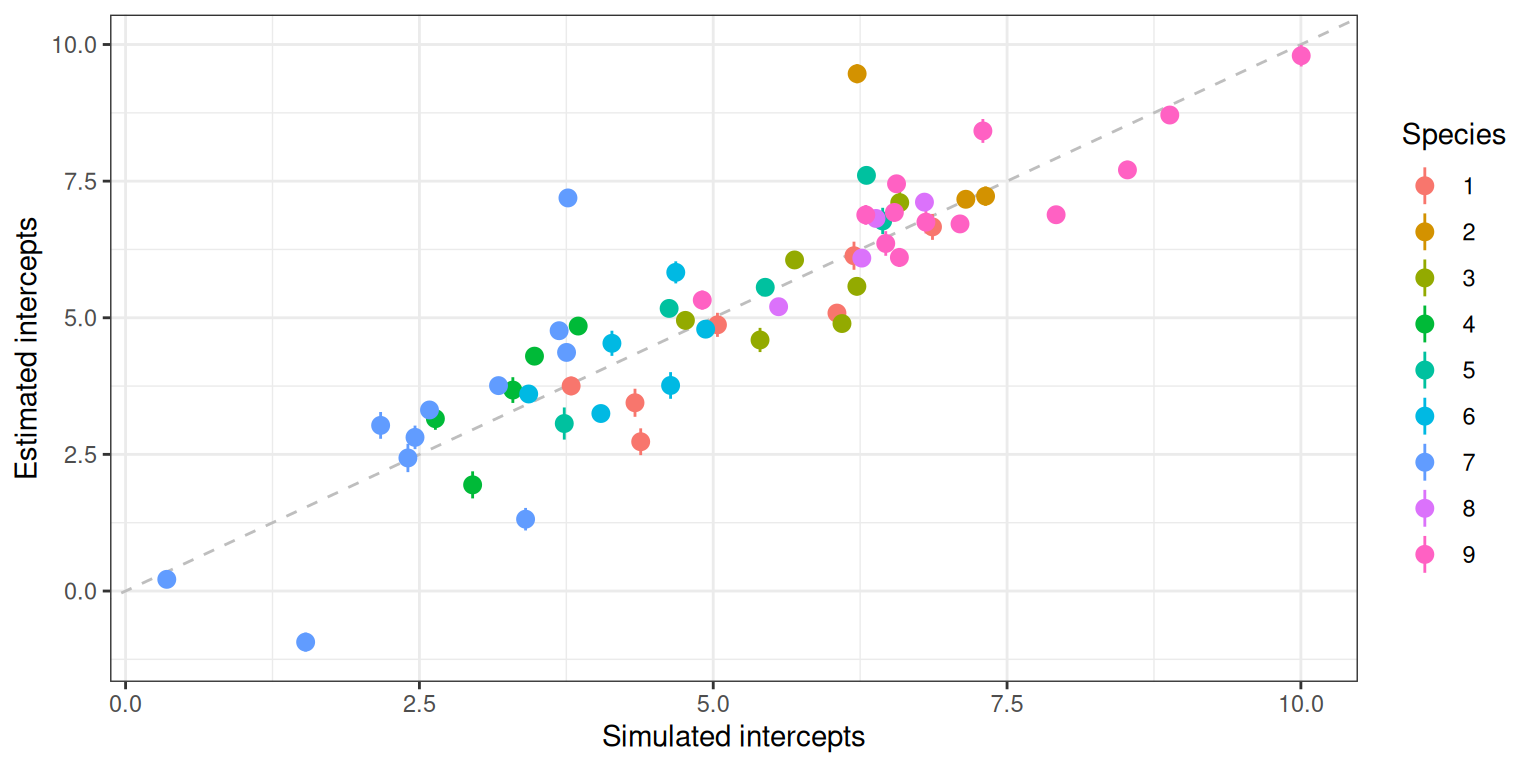
\includegraphics{lpiworkflow_files/figure-pdf/inference pop sim data-1.pdf}\end{minipage}%
%
\begin{minipage}{0.50\linewidth}
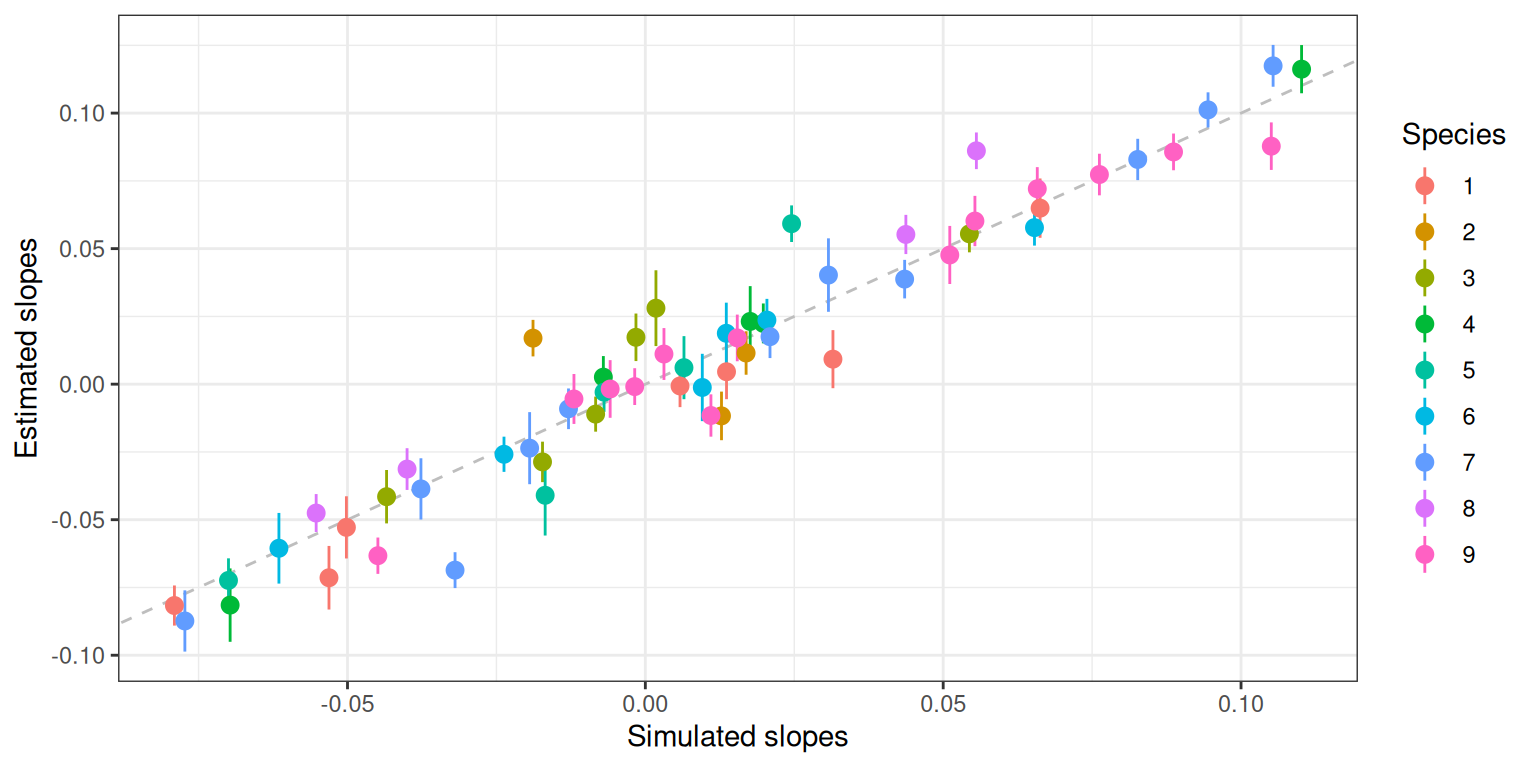
\includegraphics{lpiworkflow_files/figure-pdf/inference pop sim data-2.pdf}\end{minipage}%

\end{figure}%

What if the model did not do a good job at recovering our parameters?
Then we should likely adjust our sample size up and/or our error lower
to make sure it is can (as a basic code test).

But what if the model can recover parameters only at sample sizes much
higher than our data (or at error sizes much lower than our data)? Then
we would need to take this important information forward in our analysis
and be careful in how we interpret estimates from our model fit to
empirical data (as we have a hint at this stage that getting robust
estimates from our data and model together may be difficult, but we do
not know the actual values of our parameters -- including error and
variance parameters -- from our empirical data so we cannot be sure of
whether we may have these issues yet).

For now, we also take a look at how model fits look against the
simulated data (error bars and ribbon represent the 95\% uncertainty
intervals):

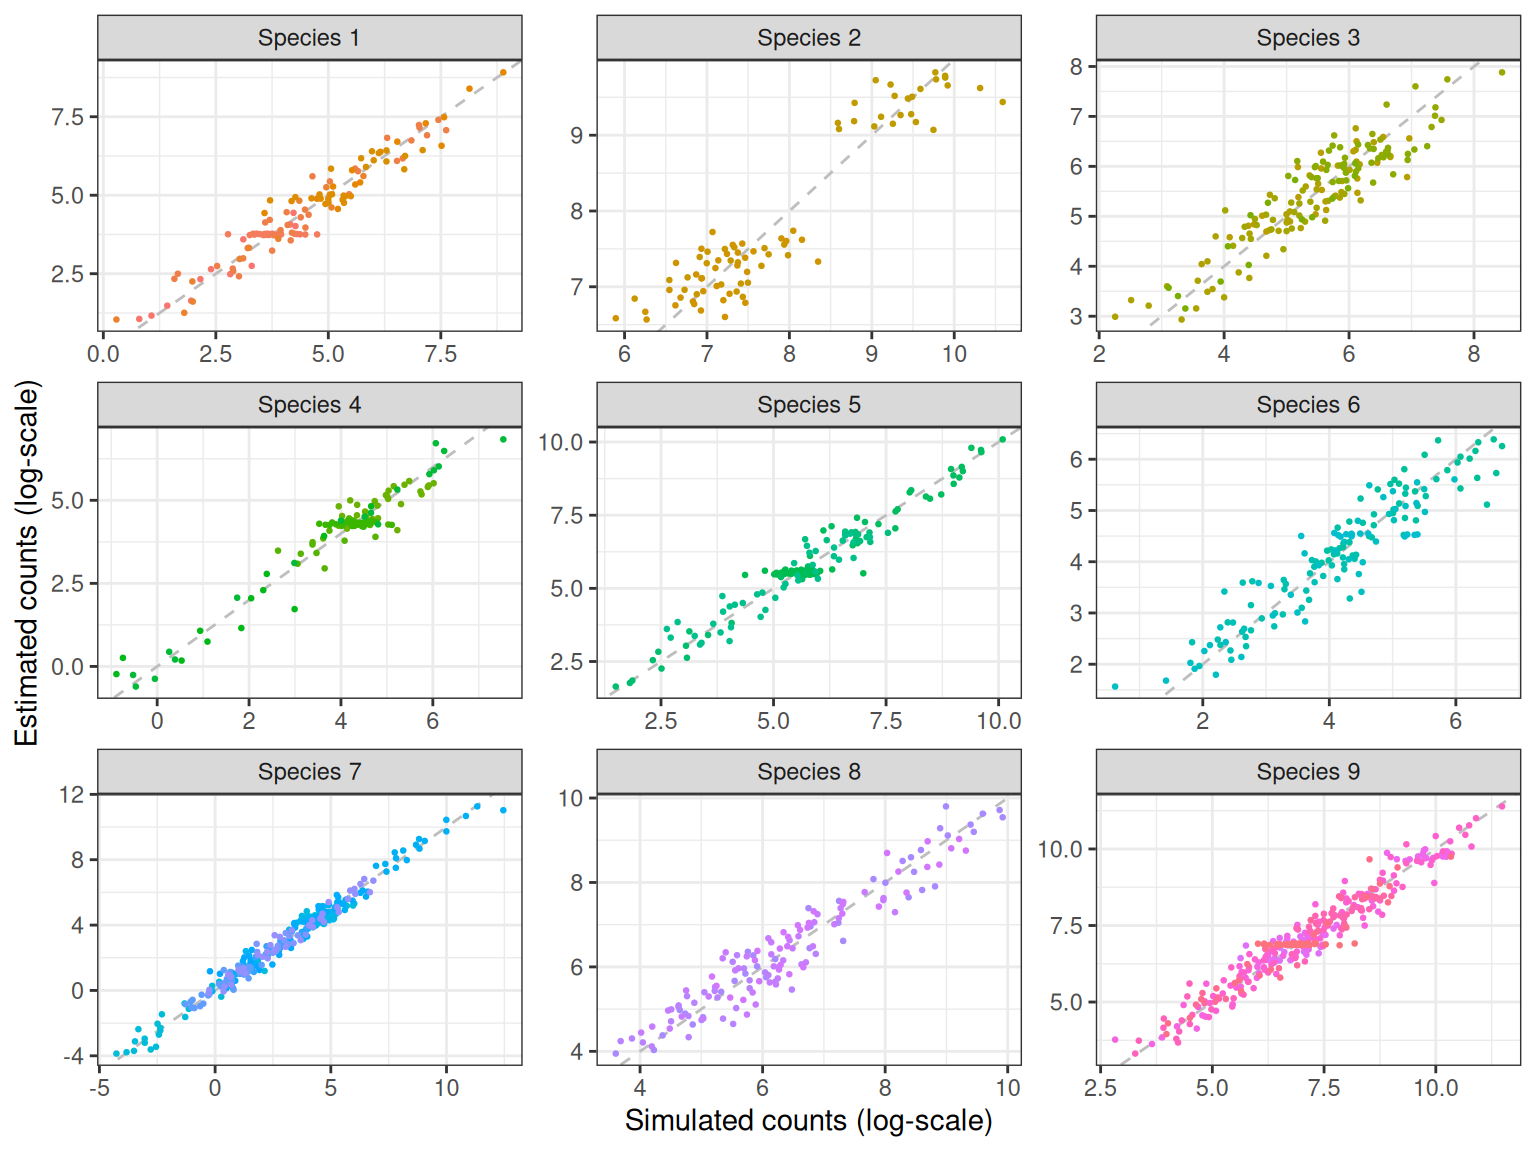
\includegraphics{lpiworkflow_files/figure-pdf/retro sim data-1.pdf}

\includegraphics{lpiworkflow_files/figure-pdf/retro sim data time-1.pdf}

These look pretty good, so we move onto the next step.

\section{Step 4: Fit model to empirical
data}\label{step-4-fit-model-to-empirical-data}

Now that we have designed our question, built our model for it, and
tested our model on simulated data, we can fit the model to our
empirical data. We start by some basic clean-up of the dataframe so we
have years in one column.

\begin{Shaded}
\begin{Highlighting}[]
\NormalTok{lpi\_subset }\OtherTok{\textless{}{-}}\NormalTok{ lpi\_subset[, }\FunctionTok{c}\NormalTok{(}\StringTok{"ID"}\NormalTok{, }\StringTok{"Genus"}\NormalTok{, }\StringTok{"Species"}\NormalTok{, }\StringTok{"Country"}\NormalTok{, }\StringTok{"Units"}\NormalTok{, }
                             \FunctionTok{paste0}\NormalTok{(}\StringTok{"X"}\NormalTok{, }\DecValTok{1950}\SpecialCharTok{:}\DecValTok{2020}\NormalTok{))]}
\NormalTok{lpi\_subset}\SpecialCharTok{$}\NormalTok{genus\_species }\OtherTok{\textless{}{-}} \FunctionTok{paste}\NormalTok{(lpi\_subset}\SpecialCharTok{$}\NormalTok{Genus, lpi\_subset}\SpecialCharTok{$}\NormalTok{Species)}

\NormalTok{lpi\_subset\_rsh }\OtherTok{\textless{}{-}} 
  \FunctionTok{reshape}\NormalTok{(lpi\_subset, }\AttributeTok{direction =} \StringTok{"long"}\NormalTok{, }\AttributeTok{idvar =} \StringTok{"ID"}\NormalTok{,}
          \AttributeTok{varying =}  \FunctionTok{paste0}\NormalTok{(}\StringTok{"X"}\NormalTok{, }\DecValTok{1950}\SpecialCharTok{:}\DecValTok{2020}\NormalTok{), }\AttributeTok{v.names =} \FunctionTok{c}\NormalTok{(}\StringTok{"value"}\NormalTok{), }
          \AttributeTok{timevar =} \StringTok{"year"}\NormalTok{, }\AttributeTok{times =} \DecValTok{1950}\SpecialCharTok{:}\DecValTok{2020}\NormalTok{)}
\NormalTok{lpi\_subset\_rsh }\OtherTok{\textless{}{-}}\NormalTok{ lpi\_subset\_rsh[lpi\_subset\_rsh}\SpecialCharTok{$}\NormalTok{value }\SpecialCharTok{!=} \StringTok{"NULL"}\NormalTok{,]}
\NormalTok{lpi\_subset\_rsh}\SpecialCharTok{$}\NormalTok{value }\OtherTok{\textless{}{-}} \FunctionTok{as.numeric}\NormalTok{(lpi\_subset\_rsh}\SpecialCharTok{$}\NormalTok{value)}
\end{Highlighting}
\end{Shaded}

The values in the database are not necessarily in the same units, so we
subset to units related to absolute population sizes, which is what we
have mostly been thinking of (some units are in density and we would
need to build our model to incorporate those, but here we start first
with a simpler model and can build up later). We take a quick look at
the data to make sure it looks reasonable based on our domain knowledge.

\begin{Shaded}
\begin{Highlighting}[]
\NormalTok{units\_to\_keep }\OtherTok{\textless{}{-}} \FunctionTok{c}\NormalTok{(}\StringTok{"Estimate {-} entire population"}\NormalTok{, }\StringTok{"Estimate {-} entire population (August)"}\NormalTok{, }
                   \StringTok{"Individual"}\NormalTok{, }\StringTok{"individuals"}\NormalTok{, }\StringTok{"Individuals"}\NormalTok{, }\StringTok{"Number of adults"}\NormalTok{, }
                   \StringTok{"number of individuals"}\NormalTok{, }\StringTok{"Number of individuals"}\NormalTok{, }\StringTok{"Number of Individuals"}\NormalTok{, }
                   \StringTok{"Number of rhinos"}\NormalTok{, }\StringTok{"numbers of indviduals"}\NormalTok{, }\StringTok{"population estimate"}\NormalTok{, }
                   \StringTok{"Population estimate"}\NormalTok{, }\StringTok{"Population estimate (individuals)"}\NormalTok{, }
                   \StringTok{"Population estimates"}\NormalTok{, }\StringTok{"Total population size"}\NormalTok{)}

\NormalTok{lpi\_subset\_rsh }\OtherTok{\textless{}{-}}\NormalTok{ lpi\_subset\_rsh[lpi\_subset\_rsh}\SpecialCharTok{$}\NormalTok{Units }\SpecialCharTok{\%in\%}\NormalTok{ units\_to\_keep,]}

\FunctionTok{ggplot}\NormalTok{(}\AttributeTok{data =}\NormalTok{ lpi\_subset\_rsh) }\SpecialCharTok{+}
  \FunctionTok{geom\_line}\NormalTok{(}\FunctionTok{aes}\NormalTok{(}\AttributeTok{x =}\NormalTok{ year, }\AttributeTok{y =}\NormalTok{ value, }
                \AttributeTok{group =} \FunctionTok{paste0}\NormalTok{(genus\_species, ID),}
                \AttributeTok{color =}\NormalTok{ genus\_species)) }\SpecialCharTok{+}
  \FunctionTok{scale\_color\_manual}\NormalTok{(}\AttributeTok{values =} \FunctionTok{hcl.colors}\NormalTok{(}\DecValTok{14}\NormalTok{, }\AttributeTok{palette =} \StringTok{"Dark2"}\NormalTok{),}
                     \AttributeTok{breaks =} \FunctionTok{unique}\NormalTok{(lpi\_subset\_rsh}\SpecialCharTok{$}\NormalTok{genus\_species)[}\FunctionTok{order}\NormalTok{(}\FunctionTok{unique}\NormalTok{(lpi\_subset\_rsh}\SpecialCharTok{$}\NormalTok{genus\_species))]) }\SpecialCharTok{+}
  \FunctionTok{theme\_bw}\NormalTok{() }\SpecialCharTok{+}
  \FunctionTok{labs}\NormalTok{(}\AttributeTok{x =} \StringTok{\textquotesingle{}Year\textquotesingle{}}\NormalTok{, }\AttributeTok{y =} \StringTok{\textquotesingle{}Observed counts\textquotesingle{}}\NormalTok{)}
\FunctionTok{ggplot}\NormalTok{(}\AttributeTok{data =}\NormalTok{ lpi\_subset\_rsh[lpi\_subset\_rsh}\SpecialCharTok{$}\NormalTok{value }\SpecialCharTok{!=} \DecValTok{0}\NormalTok{,]) }\SpecialCharTok{+}
  \FunctionTok{geom\_line}\NormalTok{(}\FunctionTok{aes}\NormalTok{(}\AttributeTok{x =}\NormalTok{ year, }\AttributeTok{y =} \FunctionTok{log}\NormalTok{(value), }
                \AttributeTok{group =} \FunctionTok{paste0}\NormalTok{(genus\_species, ID),}
                \AttributeTok{color =}\NormalTok{ genus\_species)) }\SpecialCharTok{+}
  \FunctionTok{scale\_color\_manual}\NormalTok{(}\AttributeTok{values =} \FunctionTok{hcl.colors}\NormalTok{(}\DecValTok{14}\NormalTok{, }\AttributeTok{palette =} \StringTok{"Dark2"}\NormalTok{),}
                     \AttributeTok{breaks =} \FunctionTok{unique}\NormalTok{(lpi\_subset\_rsh}\SpecialCharTok{$}\NormalTok{genus\_species)[}\FunctionTok{order}\NormalTok{(}\FunctionTok{unique}\NormalTok{(lpi\_subset\_rsh}\SpecialCharTok{$}\NormalTok{genus\_species))]) }\SpecialCharTok{+}
  \FunctionTok{theme\_bw}\NormalTok{() }\SpecialCharTok{+}
  \FunctionTok{labs}\NormalTok{(}\AttributeTok{x =} \StringTok{\textquotesingle{}Year\textquotesingle{}}\NormalTok{, }\AttributeTok{y =} \StringTok{\textquotesingle{}Observed counts (log{-}scale)\textquotesingle{}}\NormalTok{, }\AttributeTok{color =} \StringTok{"Species"}\NormalTok{)}
\end{Highlighting}
\end{Shaded}

\begin{figure}

\begin{minipage}{\linewidth}
\includegraphics{lpiworkflow_files/figure-pdf/units-1.pdf}\end{minipage}%
\newline
\begin{minipage}{\linewidth}
\includegraphics{lpiworkflow_files/figure-pdf/units-2.pdf}\end{minipage}%

\end{figure}%

Now, we make a few final adjustments and fit the model:

\begin{Shaded}
\begin{Highlighting}[]
\NormalTok{runmodel }\OtherTok{\textless{}{-}} \ConstantTok{FALSE}

\CommentTok{\# We now also find we have counts of 0, which is tricky for our approach }
\CommentTok{\#(as we cannot evaluate log(0)), we would also flag this to return. }
\CommentTok{\# As we iteratively improve the model, we would need to consider what }
\CommentTok{\# processes generate these zeroes, and include them in our model.}
\NormalTok{lpi\_subset\_rsh }\OtherTok{\textless{}{-}}\NormalTok{ lpi\_subset\_rsh[lpi\_subset\_rsh}\SpecialCharTok{$}\NormalTok{value }\SpecialCharTok{!=} \DecValTok{0}\NormalTok{,] }

\NormalTok{popids }\OtherTok{\textless{}{-}} \FunctionTok{data.frame}\NormalTok{(}\AttributeTok{ID =} \FunctionTok{unique}\NormalTok{(lpi\_subset\_rsh}\SpecialCharTok{$}\NormalTok{ID), }
                     \AttributeTok{popid\_num =} \DecValTok{1}\SpecialCharTok{:}\FunctionTok{length}\NormalTok{(}\FunctionTok{unique}\NormalTok{(lpi\_subset\_rsh}\SpecialCharTok{$}\NormalTok{ID)))}
\NormalTok{spids }\OtherTok{\textless{}{-}} \FunctionTok{data.frame}\NormalTok{(}\AttributeTok{genus\_species =} \FunctionTok{unique}\NormalTok{(lpi\_subset\_rsh}\SpecialCharTok{$}\NormalTok{genus\_species), }
                    \AttributeTok{spid\_num =} \DecValTok{1}\SpecialCharTok{:}\FunctionTok{length}\NormalTok{(}\FunctionTok{unique}\NormalTok{(lpi\_subset\_rsh}\SpecialCharTok{$}\NormalTok{genus\_species)))}

\NormalTok{lpi\_subset\_rsh }\OtherTok{\textless{}{-}} \FunctionTok{merge}\NormalTok{(lpi\_subset\_rsh, spids)}
\NormalTok{lpi\_subset\_rsh }\OtherTok{\textless{}{-}} \FunctionTok{merge}\NormalTok{(lpi\_subset\_rsh, popids)}

\NormalTok{spid\_perpop }\OtherTok{\textless{}{-}} \FunctionTok{unique}\NormalTok{(lpi\_subset\_rsh[}\FunctionTok{c}\NormalTok{(}\StringTok{"popid\_num"}\NormalTok{, }\StringTok{"spid\_num"}\NormalTok{)])}
\NormalTok{spid\_perpop }\OtherTok{\textless{}{-}}\NormalTok{ spid\_perpop[}\FunctionTok{order}\NormalTok{(spid\_perpop}\SpecialCharTok{$}\NormalTok{popid\_num),]}

\NormalTok{data }\OtherTok{\textless{}{-}} \FunctionTok{list}\NormalTok{(}
  \AttributeTok{N =} \FunctionTok{nrow}\NormalTok{(lpi\_subset\_rsh),}
  \AttributeTok{Nsp =} \FunctionTok{max}\NormalTok{(spids}\SpecialCharTok{$}\NormalTok{spid\_num),}
  \AttributeTok{Npop =} \FunctionTok{max}\NormalTok{(popids}\SpecialCharTok{$}\NormalTok{popid\_num),}
  \AttributeTok{y =}\NormalTok{ lpi\_subset\_rsh}\SpecialCharTok{$}\NormalTok{value,}
  \AttributeTok{year =}\NormalTok{ lpi\_subset\_rsh}\SpecialCharTok{$}\NormalTok{year,}
  \AttributeTok{spid\_perpop =}\NormalTok{ spid\_perpop}\SpecialCharTok{$}\NormalTok{spid\_num,}
  \AttributeTok{popid =}\NormalTok{ lpi\_subset\_rsh}\SpecialCharTok{$}\NormalTok{popid\_num}
\NormalTok{)}

\ControlFlowTok{if}\NormalTok{(runmodel)\{}
\NormalTok{  fit }\OtherTok{\textless{}{-}} \FunctionTok{stan}\NormalTok{(}\AttributeTok{file =} \StringTok{"\textasciitilde{}/projects/forecastflows/analyses/stan/model1\_nc2.stan"}\NormalTok{,}
            \AttributeTok{data =}\NormalTok{ data,  }\AttributeTok{iter=}\DecValTok{4000}\NormalTok{, }\AttributeTok{warmup=}\DecValTok{3000}\NormalTok{, }\AttributeTok{cores =} \DecValTok{4}\NormalTok{, }\AttributeTok{seed =} \DecValTok{20012029}\NormalTok{)}
  \FunctionTok{saveRDS}\NormalTok{(fit, }\AttributeTok{file =} \FunctionTok{file.path}\NormalTok{(wd, }\StringTok{"output/fit/truedatafit.rds"}\NormalTok{))}
\NormalTok{\}}\ControlFlowTok{else}\NormalTok{\{}
\NormalTok{  fit }\OtherTok{\textless{}{-}} \FunctionTok{readRDS}\NormalTok{(}\AttributeTok{file =} \FunctionTok{file.path}\NormalTok{(wd, }\StringTok{"output/fit/truedatafit.rds"}\NormalTok{))}
\NormalTok{\}}
\end{Highlighting}
\end{Shaded}

Here we finally get to see how our model performs on the empirical data
and are a step closer to answering our question, but we also start to
notice some differences in our empirical data from our simulated data.
In preparing our data for the model, we realize we have quite different
amplitudes of variations across populations and species (on a
log-scale), e.g.~for blue wildebeest (each color represents a different
population):

\includegraphics{lpiworkflow_files/figure-pdf/unnamed-chunk-4-1.pdf}

Our model may accommodate this, as we have allowed different populations
to have different intercepts (starting population sizes), but the scale
of this variation is much larger than we simulated so we would again
want to flag this and check how our model performs with these data.

\section{Step 5: Retrodictive and related
checks}\label{step-5-retrodictive-and-related-checks}

Now we use our fitted model parameters to generate predictions, and
compare them to observations. This is similar to the simulating data
step above, but differs in two major ways: (1) we simulate from the
parameters estimated by the model fit to the empirical data (versus
coming up with them based on our expert knowledge) and (2) we need to
check across many predictions from the model to understand the full
uncertainty of the model (and not just one draw from the model).

Here we start by visually comparing the posterior predictive
distribution of the predicted counts (across all species and
populations, red line) to observed data (black dashed line):

\includegraphics{lpiworkflow_files/figure-pdf/unnamed-chunk-5-1.pdf}

We can also look at some posterior replications separately:

\includegraphics{lpiworkflow_files/figure-pdf/unnamed-chunk-6-1.pdf}

We then examine, by species, how well predictions from the model compare
to the observed data; this is similar to many plots where we simply want
to see how well the model seems to predict the data.

\includegraphics{lpiworkflow_files/figure-pdf/unnamed-chunk-7-1.pdf}

To evaluate our model more precisely, we need to check how the model
predicts the data on finer scales. So we start by examining some species
separately, e.g.~here the African bush elephant (each color within a
country represents a different population):

\includegraphics{lpiworkflow_files/figure-pdf/unnamed-chunk-8-1.pdf}

Focusing on populations in South Africa, we see some places where the
linear model appears to fit reasonably well (ID 7673), but also one
population where it does not appear as a very good fit (ID 10010).

\includegraphics{lpiworkflow_files/figure-pdf/unnamed-chunk-9-1.pdf}

The three populations are measured in the same units, but are very
different in their sizes (ranging from a few hundred individuals to more
than 10000), thus they likely represent populations measured across
different spatial scales.

The same holds for other species and other countries, e.g.~the blue
wildebeest in Tanzania:

\includegraphics{lpiworkflow_files/figure-pdf/unnamed-chunk-10-1.pdf}

The four populations are also measured in the same basic units, but
represent likely represent very different populations, spanning ones in
small parks that cannot migrate to the large migrating herds (e.g.,
Serengeti Masai-Mara), though gathering additional metadata to fully
check this would be another important component to add to our workflow
for these data.

\section{Inference}\label{inference}

Once we are confident with our model (which is not truly the case here),
we can look at the parameter values and check what the overall and
species trends appear to be:

\includegraphics{lpiworkflow_files/figure-pdf/unnamed-chunk-11-1.pdf}

\section{Feedbacks}\label{feedbacks}

At this point, we would have a lot of ideas of ways to improve this
model that we would want to follow up on, including (but not limited to)
questioning our assumption of one observational error \(\sigma\) for all
populations, how we model population trends (e.g., there are many ways
to model abundance), and (relatedly) our linearity assumption. One
possibility would be to move to a non-linear regression, and use a more
flexible model that would allow population numbers to stabilize, such as
shown using a logistic model for one wildbeest population in Tanzania:

\begin{Shaded}
\begin{Highlighting}[]
\NormalTok{subset\_wildebeest }\OtherTok{\textless{}{-}}\NormalTok{ lpi\_subset\_rsh[lpi\_subset\_rsh}\SpecialCharTok{$}\NormalTok{ID }\SpecialCharTok{==} \DecValTok{5589}\NormalTok{,]}
\NormalTok{subset\_wildebeest}\SpecialCharTok{$}\NormalTok{year }\OtherTok{\textless{}{-}}\NormalTok{ subset\_wildebeest}\SpecialCharTok{$}\NormalTok{year}\DecValTok{{-}1980}
\NormalTok{gompodel }\OtherTok{\textless{}{-}} \FunctionTok{nls}\NormalTok{(}\FunctionTok{log}\NormalTok{(value) }\SpecialCharTok{\textasciitilde{}} \FunctionTok{SSlogis}\NormalTok{(year, Asym, b2, b3), }\AttributeTok{data=}\NormalTok{subset\_wildebeest)}
\NormalTok{logisfit }\OtherTok{\textless{}{-}}\FunctionTok{data.frame}\NormalTok{(}\AttributeTok{pred =} \FunctionTok{predict}\NormalTok{(gompodel, }
                                     \AttributeTok{newdata =} \FunctionTok{data.frame}\NormalTok{(}\AttributeTok{year =} \FunctionTok{seq}\NormalTok{(}\SpecialCharTok{{-}}\DecValTok{25}\NormalTok{,}\DecValTok{30}\NormalTok{,}\DecValTok{1}\NormalTok{))), }
                      \AttributeTok{year =} \FunctionTok{seq}\NormalTok{(}\SpecialCharTok{{-}}\DecValTok{25}\NormalTok{,}\DecValTok{30}\NormalTok{,}\DecValTok{1}\NormalTok{))}

\FunctionTok{ggplot}\NormalTok{(}\AttributeTok{data =}\NormalTok{ lpi\_subset\_rsh[lpi\_subset\_rsh}\SpecialCharTok{$}\NormalTok{ID }\SpecialCharTok{==} \DecValTok{5589}\NormalTok{,]) }\SpecialCharTok{+}
  \FunctionTok{facet\_wrap}\NormalTok{( }\SpecialCharTok{\textasciitilde{}}\NormalTok{ ID, }\AttributeTok{scales =} \StringTok{"free\_y"}\NormalTok{) }\SpecialCharTok{+}
  \FunctionTok{geom\_point}\NormalTok{(}\FunctionTok{aes}\NormalTok{(}\AttributeTok{x =}\NormalTok{ year, }\AttributeTok{y =}\NormalTok{ value),}
             \AttributeTok{size =} \FloatTok{0.7}\NormalTok{, }\AttributeTok{color =} \StringTok{"grey"}\NormalTok{) }\SpecialCharTok{+} 
  \FunctionTok{geom\_line}\NormalTok{(}\FunctionTok{aes}\NormalTok{(}\AttributeTok{x =}\NormalTok{ year, }\AttributeTok{y =}\NormalTok{ value),}
             \AttributeTok{linewidth =} \FloatTok{0.3}\NormalTok{, }\AttributeTok{color =} \StringTok{"grey"}\NormalTok{) }\SpecialCharTok{+} 
  \FunctionTok{geom\_line}\NormalTok{(}\FunctionTok{aes}\NormalTok{(}\AttributeTok{x =}\NormalTok{ year }\SpecialCharTok{+} \DecValTok{1980}\NormalTok{, }\AttributeTok{y =} \FunctionTok{exp}\NormalTok{(pred)),}
            \AttributeTok{linewidth =} \FloatTok{0.5}\NormalTok{, }\AttributeTok{data =}\NormalTok{ logisfit, }\AttributeTok{linetype =} \StringTok{\textquotesingle{}dashed\textquotesingle{}}\NormalTok{) }\SpecialCharTok{+}
  \FunctionTok{theme\_bw}\NormalTok{() }\SpecialCharTok{+} 
  \FunctionTok{labs}\NormalTok{(}\AttributeTok{y =} \StringTok{\textquotesingle{}Counts\textquotesingle{}}\NormalTok{, }\AttributeTok{x =} \StringTok{\textquotesingle{}Year\textquotesingle{}}\NormalTok{)}
\end{Highlighting}
\end{Shaded}

\includegraphics{lpiworkflow_files/figure-pdf/unnamed-chunk-12-1.pdf}

We also have seen variability in population trends within species (e.g.,
two apparently increasing populations and two apparently decreasing
populations in Tanzania), so we would want to think a lot more about how
we scale up from population to species to capture this variation in a
way that is most useful to our question. For example, may want to think
about adding country, which may capture differences in efforts related
to conservation and thus predict trends (or we may have better metrics
of what drives these trends, but given our global aim, we would ideally
need the predictor for most/all populations) and we may want to think
about how or if we partially pool species and populations within species
(potentially using models other than a normal distribution for pooling).
As we address these potential problems, we would likely begin to add in
more countries, species, and populations.

We expect scaling up to more countries, species and populations may
cause us to think carefully about the data we have in hand and our
approach versus the question we aimed to answer. While many recent
papers treat the LPI data as (effectively) a well stratified and
randomized sample or even a good census, the LPI data is clearly
neither. Thus, models that try to deal with such uneven sampling and
build in more of the structure of data would be more appropriate. For
example, most models for election forecasts now include regularization
via partial pooling, post-stratification and other methods designed to
adjust for the fact that many polls are `non-representative.' Such
non-representative polls may be very similar to LPI data. Our model
includes some regularization via partial pooling, but we may need much
more of an observational model added to our population demography model
to accommodate the uneven sampling. Estimates from such a model may be
more uncertain, but likely also more correct given our combination of
question and data.

This may lead us to realize we really don't have great data for this
question and we would then need to prioritize better data collection
efforts if we want good estimates to answer this question.

\section{The full process}\label{the-full-process}

The small workflow we show here may seem like extra work to those who
have not used it, and it is compared to many ecological workflows in
practice. We argue that the extra effort is worth it given the critical
questions we are addressing, and also that the process becomes much
quicker with practice. The first time may be slow, but the resulting
model will be better for it (even if it is still arguably simple, as the
one we show here is), but the following uses of this iterative workflow
will go faster and very likely yield improved models.




\end{document}
